\subsection{Power Macromodel for Combinational Logic}
To validate the accuracy of the power macromodel proposed in~\cite{Najm2000_2}, we will generate multiple sequences of input training vectors, derive an accurate power estimate from PrimeTime, and use the statistics ($P_{in}, D_{in}, SC_{in}, D_{out}$) associated with each sequence to train the macromodel. We will then generate a separate set of sequences which will be used to test the macromodel's accuracy as compared to the PrimeTime power estimate.

The combinational circuits used in this study were the following ISCAS 85 benchmark circuits:

\begin{itemize}
	\item \em{c17}: 6 NAND gates
	\item \em{c432}: 27-channel interrupt controller
	\item \em{c499}: 32-bit SEC
	\item \em{c880}: 8-bit ALU
	\item \em{c1908}: 16-bit SEC/DED
	\item \em{c2670}: 12-bit ALU
	\item \em{c6288}: 16x16 multiplier
	\item \em{c7552}: 32-bit adder/comparator 
\end{itemize}

The training and testing datasets consisted of 300 sequences of 30 vectors. They were run through the DUT using RTL simulation and post-PAR gate-level simulation. The gate-level simulations were used to derive switching activity files which when passed to PrimeTime PX gave a power estimate for a given sequence. Using the input and output vectors, and the power estimate from PrimeTime the 4 following power macromodels were constructed:

\begin{itemize}
	\item \em{4D Table}: A simple map from a $P_{in}, D_{in}, SC_{in}, D_{out}$ vector to a power estimate.
	\item \em{Linear Model}: Coefficients were derived for an equation of the form $c_0 + c_1 P_{in} + c_2 D_{in} + c_3 SC_{in} + c_4 D_{out}$ using least squares regression. (5 coefficients)
	\item \em{Quadratic Model}: Coefficients were derived for an equation consisting of the linear terms, but also cross terms and self-squared terms using least squares regression. (15 coefficients)
	\item \em{Cubic Model}: Added triplet cross terms and self-cubed terms. (35 coefficients)
\end{itemize}

Once the models were constructed and trained using the training dataset, they were used to make predictions on the testing dataset.

4D table prediction involves interpolating new ($P_{in}, D_{in}, SC_{in}, D_{out}$) vectors on the training dataset: if interpolation wasn't possible due to the testing vector being outside the convex hull of the training vectors, then the nearest neighbor's power estimate was used. Prediction on the linear, quadratic, and cubic models was performed with simple matrix multiplication of the testing vectors and the previously calculated coefficients.

Errors in the the macromodel were measured and are summarized in Figure \ref{fig:rms_error}

\begin{figure*}
	\centering
	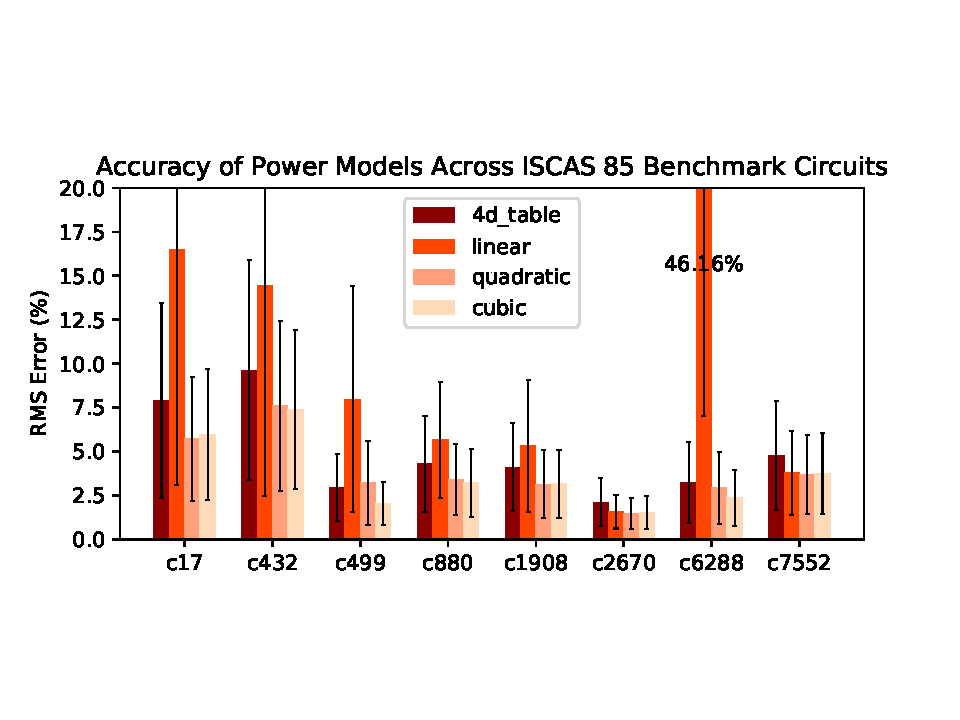
\includegraphics[clip, trim=0.5cm 2.5cm 0.5cm 2.5cm,width=0.85\textwidth,height=\textheight,keepaspectratio]{images/macromodel_rms_errors.pdf}
	\caption{RMS errors from macromodel power estimation, error bars indicate 1 SD}
	\label{fig:rms_error}
\end{figure*}


To demonstrate our idea, we will start from a simple design, RISCV-mini~\cite{riscv-mini}.
RISCV-mini implements RV32I of the User-level ISA Version 2.0~\cite{riscv-user-2.0} and
the Machine-level ISA of the Privileged Architecture Version 1.7~\cite{riscv-prev-1.7}.
RISCV-mini includes a 3-stage pipeline as well as instruction and data caches as shown
in Figure~\ref{fig:riscv_mini}, which is neither too simple nor too complex. This is designed
to validate novel ideas before applying them to more complex designs including
RocketChip~\cite{RocketChip}, Hwacha~\cite{Hwacha}, and BOOM~\cite{BOOM}.
We expect that the methodology proposed in this report will accurately predict
the power dissipation of microbenchmarks(median, multiply, qsort, towers, and vvadd) running on RISCV-mini.

\begin{figure*}
	\centering
	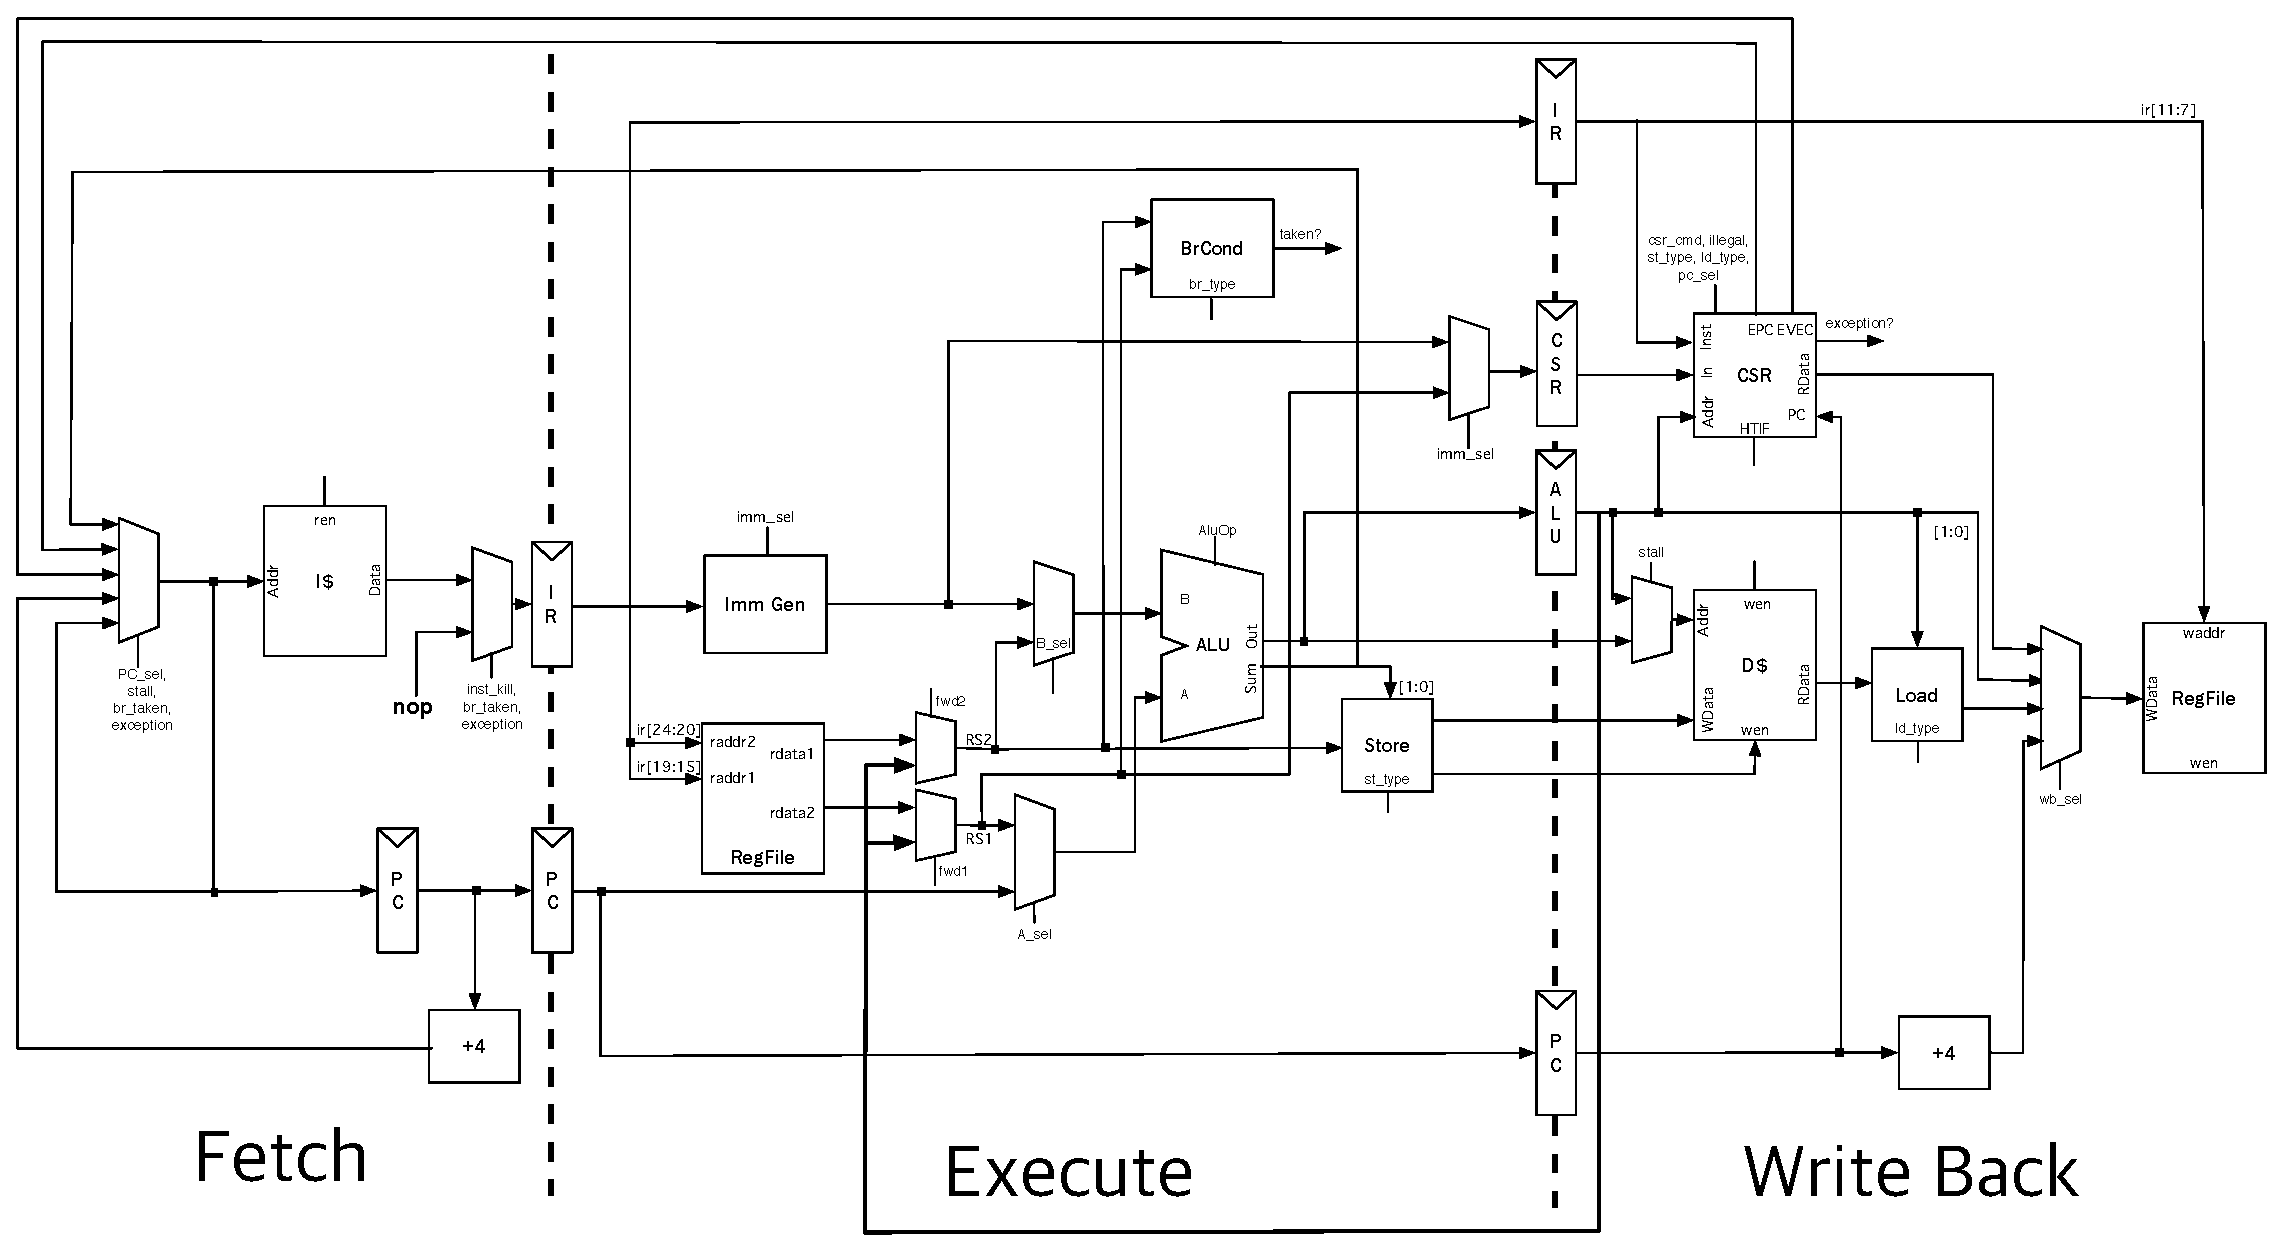
\includegraphics[width=0.85\textwidth,height=\textheight,keepaspectratio]{images/riscv_mini.pdf}
	\caption{RISCV-mini Pipeline}
	\label{fig:riscv_mini}
\end{figure*}